\section{Introduction}
\label{sec:introduction}

Choosing training data is crucial for the performance of language models (LMs) in both general-purpose and domain-specific applications \citep{brown2020languagemodelsfewshotlearners, dontstoppretrainingadapt, trainingcomputeoptimallargelanguage}. 
To date, most research on data curation has focused on creating diverse pre-training datasets to enhance model performance across a wide range of tasks \citep{sorscher2022beyond,dsir, d4, semdedup, doremi,lee2023beyond,wettig2024quratingselectinghighqualitydata,penedo2024finewebdatasetsdecantingweb,li2024datacomp,sachdeva2024train}, and while these methods have been demonstrated to work well for general pre-training, they fall short in domain-specific fine-tuning, where data relevance is crucial. This raise a key question: 
\textit{How should we, in a general purpose manner, effectively select fine-tuning data for a domain-specific target task?}

One approach is to train binary classifiers to identify relevant data. 
For example, a mathematical language model called DeepSeekMath \citep{deepseekmath} utilized OpenWebMath \citep{openwebmathopendatasethighquality}, a compilation of high-quality mathematical texts, to train a FastText classifier % \citep{enrichingWordVectorsWithSubwordInfo}
to retrieve analogous texts from the Web \citep{enrichingWordVectorsWithSubwordInfo}. 
Although effective, this method relies on the availability of large and well-annotated data sets, something that is often missing in niche tasks where relevant data are scarce. 
\begin{figure*}[t]
  \centering
  {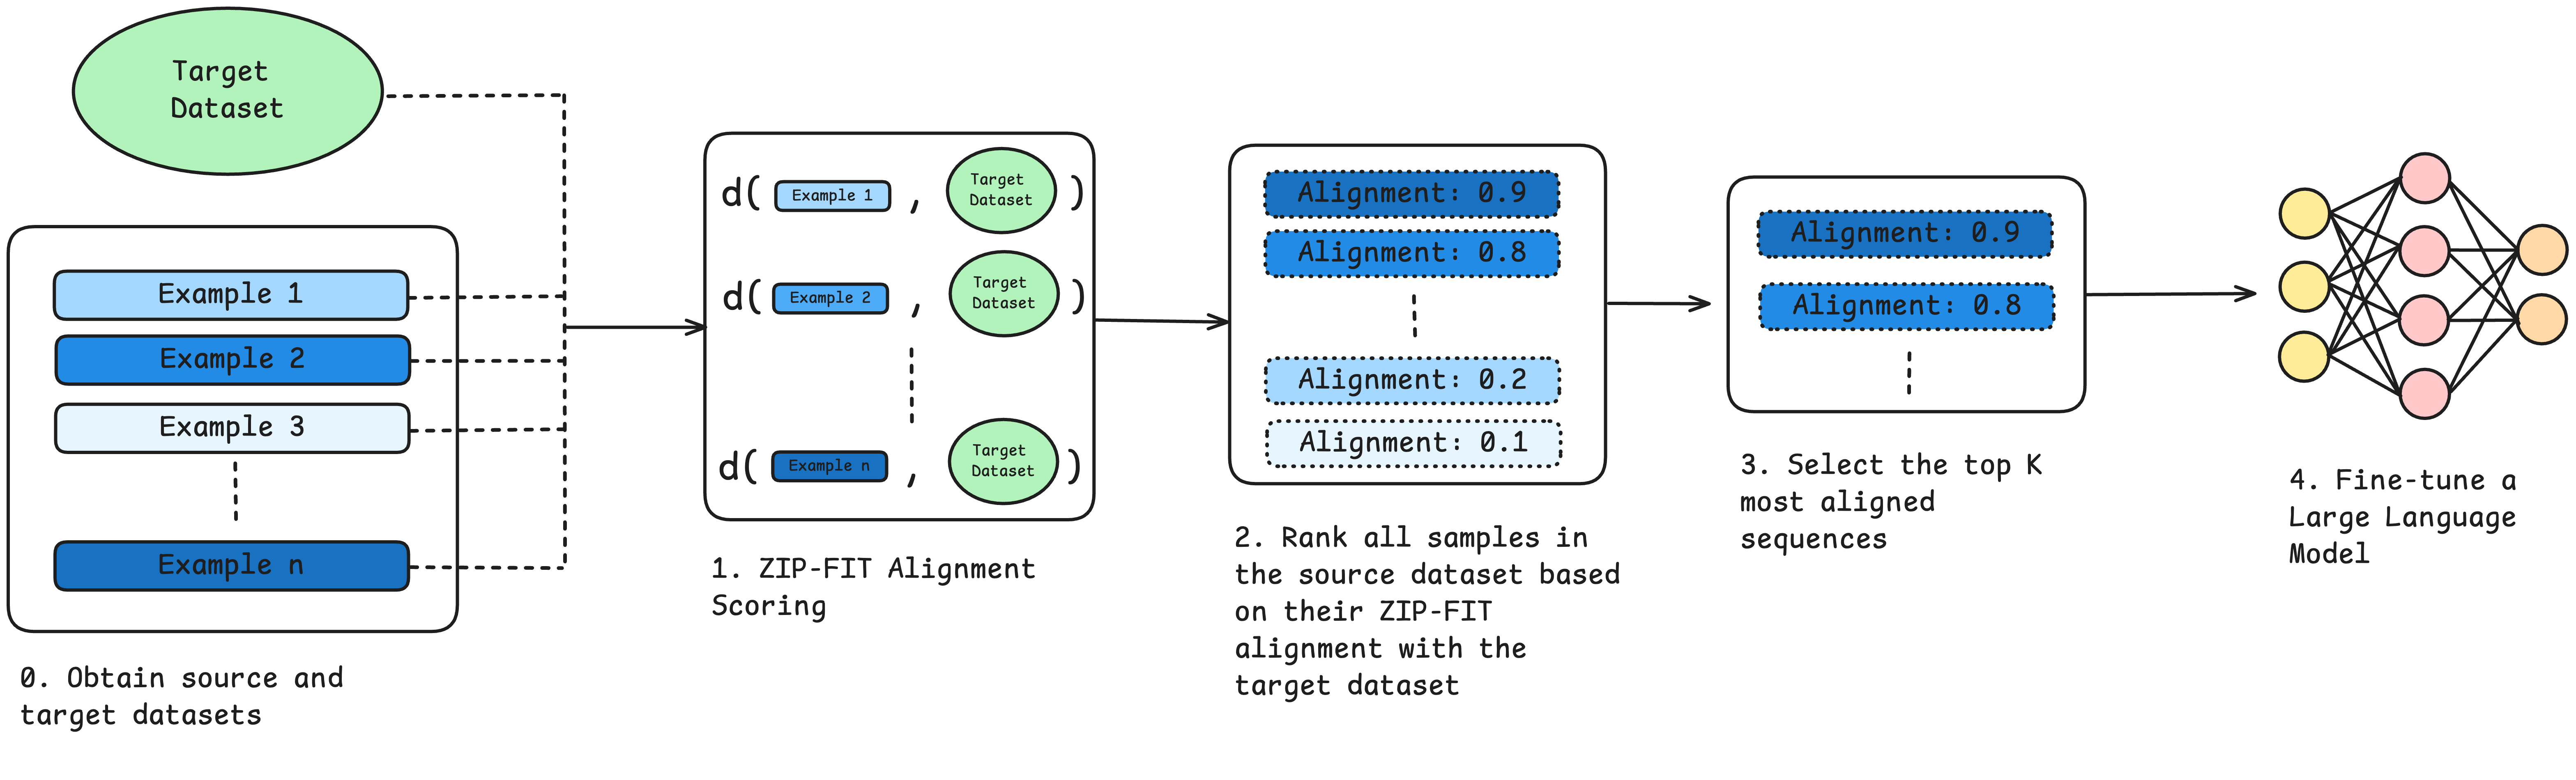
\includegraphics[width=\textwidth]{./diagrams/zip-fit-final-schematic.png}}
  \caption{\textbf{\texttt{ZIP-FIT} selects task-specific data for efficient finetuning.} 
  (0) Obtain both the source and target datasets. 
  (1) Calculate \texttt{ZIP-FIT} Alignment of each source example with the target dataset using \texttt{gzip} compression. 
  (2) Rank all source examples based on these alignment scores. 
  (3) Select the top-K most aligned examples for fine-tuning. 
  (4) Fine-tune a large language model using the selected top-K examples to improve performance on the target task.}
  \label{fig:zip-fit-vs-baselines}
\end{figure*}
\begin{figure*}[t]
  \centering
  {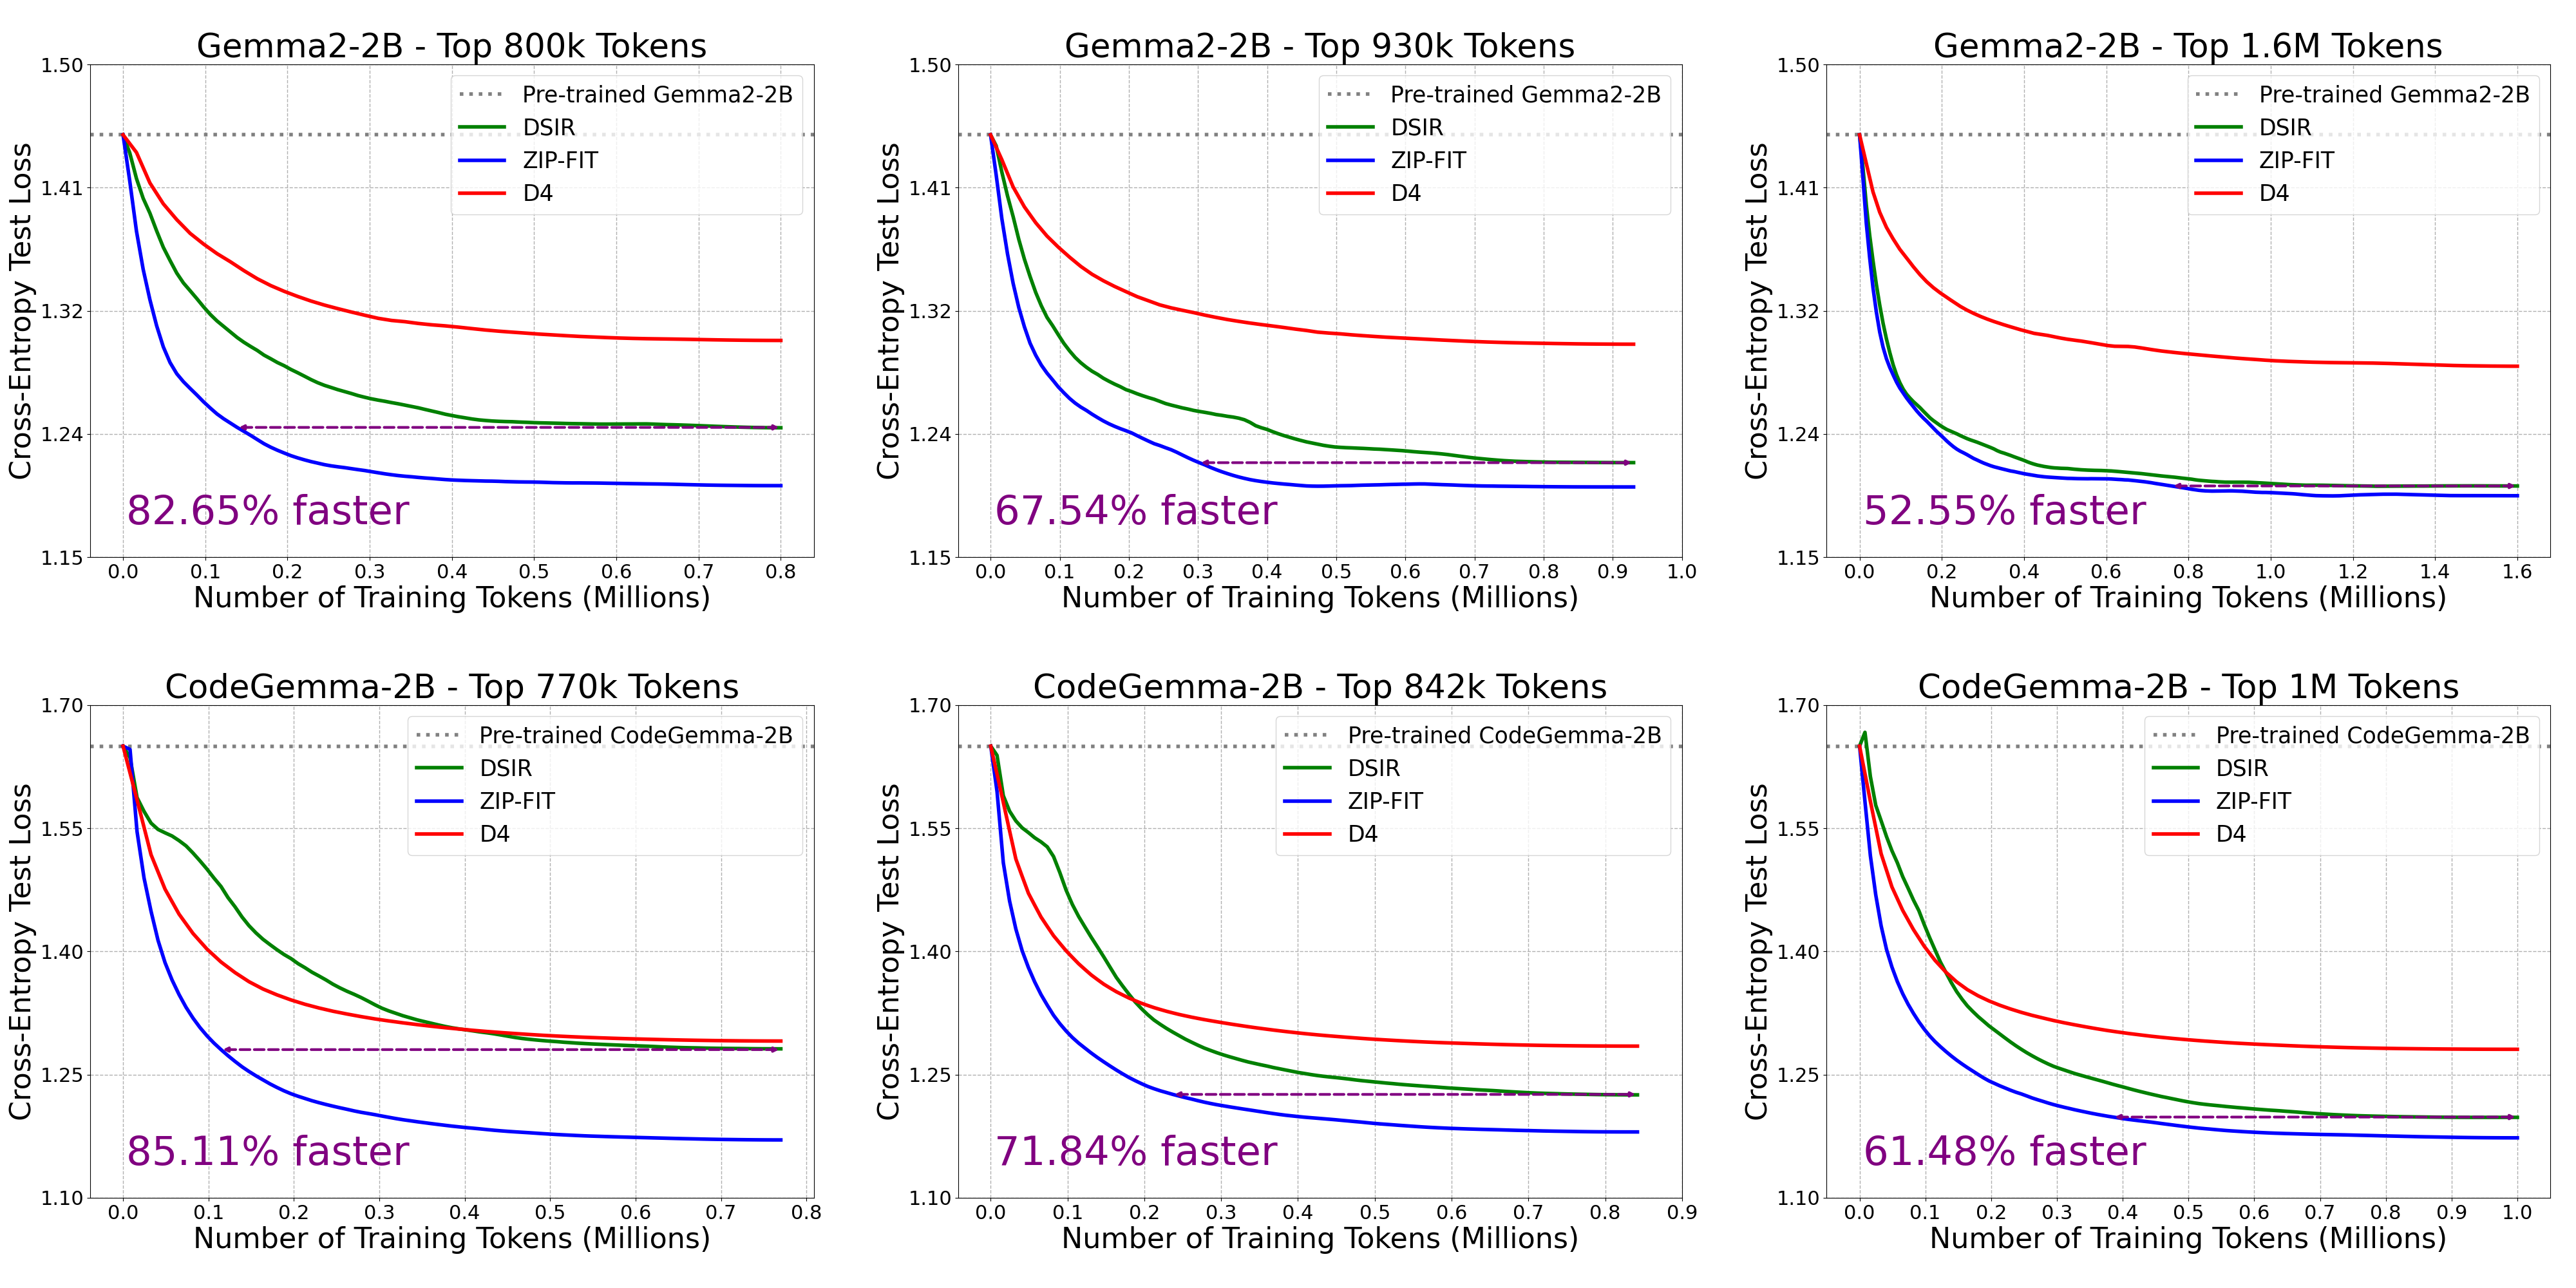
\includegraphics[width=1.0\textwidth]{./plots/code_all_models.png}}
  \caption{\textbf{Code Generation: \texttt{ZIP-FIT} accelerates cross-entropy loss reduction, even in code-specialized models like CodeGemma-2B.} The plots show cross-entropy test loss versus the number of training tokens for Gemma2-2B (top row) and CodeGemma-2B (bottom row) across different token selection sizes. \texttt{ZIP-FIT} (blue) consistently reduces loss faster than DSIR (green) and D4 (red), achieving up to $85.11\%$ speed improvement at lower token counts. These results demonstrate \texttt{ZIP-FIT}'s efficiency in data selection for fine-tuning models on code-geneation tasks.
  }
  \label{fig:code-all-models}
\end{figure*}
Another common approach is to use neural embeddings to measure the similarity between data points and a reference corpus \citep{efficientcontinualpretrainingbuilding}. 
Although this improves relevance, embedding-based methods are computationally expensive and sensitive to the choice of embedding space \citep{sgptgptsentenceembeddings}. 
Alternatively, DSIR (Data Selection via Importance Resampling) \citep{dsir} utilizes unigrams and bigrams to select data points without the need for pre-trained embeddings, with the aim of matching the hashed n-gram distributions of the target data. Although DSIR is effective in capturing direct word correlations, it may not capture structured patterns of syntax that unfold across sentences or paragraphs, such as nested function calls in code or embedded clauses in formal language translation \citep{deMoura2015lean}. Additionally, the hashing introduces noise due to collisions. These shortcomings highlight the need for alternative data selection strategies better suited to domain-specific tasks.

To address these challenges, we propose \texttt{ZIP-FIT}, a novel data selection framework that leverages the classic compression algorithm \texttt{gzip}.
Recent research suggests that language modeling and data compression are fundamentally equivalent tasks \citep{languagemodelingcompression}, and the intelligence of large language models (LLMs) is closely related to their ability to compress external corpora \citep{compressionrepresentsintelligencelinearly}. 
This insight suggests that compression algorithms can encode information in ways similar to neural networks. 
For example, \citet{jiang-etal-2023-low} found that the use of normalized compression distances for text classification outperformed traditional neural embeddings. 
Inspired by this, \texttt{ZIP-FIT} selects aligned training data with a target data set based on compression-based alignment, providing a lightweight and embedding-free method for selecting high-quality data.

% We evaluated \texttt{ZIP-FIT} across two distinct domains: Autoformalization and Python code generation. 
% We show that \texttt{ZIP-FIT} outperforms existing data selection frameworks and consistently improves model performance, particularly when evaluating cross-entropy test loss for target domains. 
% Our experiments reveal that smaller, well-aligned datasets, chosen through \texttt{ZIP-FIT}, lead to faster convergence and superior performance compared to the use of larger, less aligned data sets, underscoring the importance of quality over quantity. 
We evaluated \texttt{ZIP-FIT} in two domains: Autoformalization and Python code generation. 
\texttt{ZIP-FIT} outperforms existing data selection methods, consistently improving model performance cross-entropy test loss. 
Smaller, well-aligned datasets selected by \texttt{ZIP-FIT} lead to faster convergence and better performance than larger, less aligned datasets, highlighting the importance of data quality.

Our \textbf{contributions} are as follows:
\begin{enumerate}
    \item \textbf{Methodology:} The introduction of \texttt{ZIP-FIT}, an embedding-free data selection method based on \texttt{gzip} compression.
    \item \textbf{Superior Performance:} \texttt{ZIP-FIT} consistently outperforms leading baselines (DSIR, D4) in Autoformalization and Python code generation, achieving up to 85.1\% faster convergence and lower cross-entropy loss.
    \item \textbf{Computational Efficiency:} \texttt{ZIP-FIT} is computationally efficient, running up to 65.8\% faster than DSIR. This makes it scalable for low-resource environments without compromising performance.
\end{enumerate}
